\documentclass[titlepage]{article}
\usepackage[bottom=3cm, right=2cm, left=2cm, top=3cm]{geometry}
\usepackage{graphicx}
\usepackage{hyperref}
\usepackage{float}

\title{SFWRENG 4NL3 Assignment 1}
\author{Sumanya Gulati}
\date{20 January 2025}

\begin{document}

\begin{titlepage}
    \maketitle
\end{titlepage}

\newpage 

\tableofcontents
\listoftables
\listoffigures

\newpage

\section{Data}
\texttt{myfile.txt} is a text file that contains inaugral speeches by United States Presidents'
from George Washington to Barack Obama. The dataset was acquired from the
\href{https://www.gutenberg.org/ebooks/4938}{Project Gutenberg} collection and was downloaded 
as a Plain Text UTF-8 encoded file. \\

Prior to tokenization, the dataset was manually pre-processed which included removing the title
page, table of contents, disclaimers and such information from the beginning and the ending of 
the text file to ensure consistency and remove any characters unrelated to the actual content.\\

I chose this dataset in light of today's inaugral speech of the 47th U.S. President. I also
wanted to be able to use the script from this assignment to gather insights about how inaugral
addresses have changed over centuries and analyze whether the increased use of words like 
`immigration' and `economy' is a recent trend over the past few decades.\\

I also want to analyze if the use of words propogating sentiments of nationalism and unity
increases in years following major national of global events like the Vietnam war, 9/11, the
2008 recession, COVID-19 pandemic and more. If you would be interested in viewing the results
of these analyses, feel free to shoot me an email and I would be glad to share them (assuming,
I am actually able to get it done soon).

\section{Methodology}
This section outlines the approach employed in writing this script and explains available
normalization options while describing their use and a rationale for using them.
\subsection{Approach}
The approach I used to write this script involved breaking it down into steps and implementing 
one required step at a time, tetsing it and then moving onto the next step. I started by writing 
a skeletal script that reads a file and implements command-line argument parsing. After that,
I wrote the \texttt{tokenize\_text()} function to pattern-match the input text file and break it
into tokens, storing the result as a list.\\

The next step involved implementing the \emph{lowercase} and \emph{remove\_stopwords}
options, followed by implementing the \emph{lemmatization} and \emph{stemming} options, the
code snippets for which were copied from the lecture slides. The \texttt{visualize()} function 
was then implemented to produce first, a DataFrame (basically, a nicer table to view the output)
and then a bar plot. A trial and error approach was used to figure out if either or both axes 
should be set as a log scale and a log-log line plot was generated to compare my result with 
that of datasets obeying Zipf's law as shown in this 
\href{https://en.wikipedia.org/wiki/Zipf's_law}{Wikipedia} article.\\

Generative AI was used to resolve a logical bug and write line 12 of the script.
A search query weas employed using ChatGPT with the following prompt: \emph{
"I am trying to tokenize an input text file using regex pattern matching but some of 
my tokens in the list are preceeded by the letters, ufeff. Could this be random or is there a 
logical error in my code?"}. As outlined in the course outline, the carbon footprint of this
query is 4.32g of CO\textsubscript{2}.

\subsection{Available Options}
The following options, in any combination, can be used by the user during the text normalization 
steps:
\begin{enumerate}
    \item \texttt{--lowercase}: Change letter case
    \item \texttt{--stem}: Apply stemming
    \item \texttt{--lemmatize}: Apply lemmatization
    \item \texttt{--remove-stopwords}: Remove commonly used stopwords in the English language
    \item \texttt{--remove-numbers}: Remove numbers 
\end{enumerate}

Beyond the defined requirements, I added the option to remove numbers. Since the text file
contains speeches spanning centuries, it seemed like a fair assumption (backed by a brief look
at the raw data) that the text file contains the use of digits to write out for example, the date
or the year of the speech. I believe this is a useful option as it removes the numbers added as a 
part of the description, producing a more consistent dataset that focuses purely on the content of 
the speeches by exluding the remaining descriptive text.\\

I recognize that this option may cause unwanted issues by removing numbers that are a part of the 
actual speech or not remove numbers that are spelled out as opposed to being written ad digits.
Configuring this option to not cause these issues seems like a more complex task that would require
additional time and effort.

\section{Sample Output}
Using the \texttt{pandas} library and the DataFrame structure, a table has been created to sort 
the list of unique tokens in decreasing order along with their frequency/count.\\

Figures \ref{fig:FigTop25} and \ref{fig:FigTop25Stop} display tables showing the top 25 words and
their frequency based on the program's output. Figure \ref{fig:FigTop25} has been generated using 
all options except \texttt{--stem} and figure \ref{fig:FigTop25Stop} has been generated using only 
the \texttt{--lowercase} and \texttt{--lemmatize} options.

\begin{figure}[H]
    \centering
    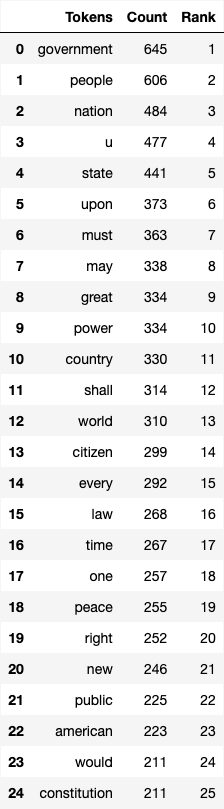
\includegraphics[width=0.27\textwidth]{figures/df_top25.png}
    \caption{Top 25 words with their count.}
    \label{fig:FigTop25}
\end{figure}

\begin{figure}[H]
    \centering
    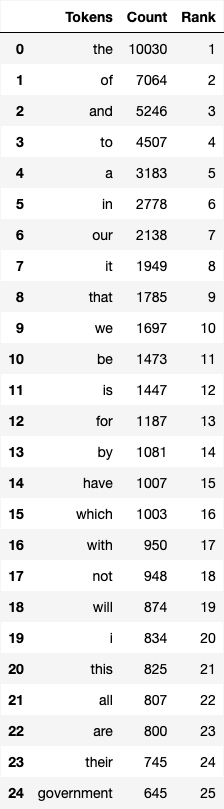
\includegraphics[width=0.27\textwidth]{figures/df_top25_stopwords.png}
    \caption{Top 25 (including stopwords) words with their count.}
    \label{fig:FigTop25Stop}
\end{figure}

Figures \ref{fig:FigLast25} and \ref{fig:FigLast25Stop} display tables showing the last 25 words and
their frequency based on the program's output. Figure \ref{fig:FigLast25} has been generated using 
all options except \texttt{--stem} and figure \ref{fig:FigLast25Stop} has been generated using only 
the \texttt{--lowercase} and \texttt{--lemmatize} options.

\begin{figure}[H]
    \centering
    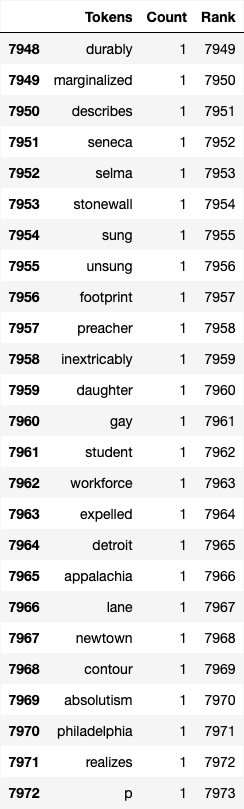
\includegraphics[width=0.35\textwidth]{figures/df_last25.png}
    \caption{Last 25 words with their count.}
    \label{fig:FigLast25}
\end{figure}

\begin{figure}[H]
    \centering
    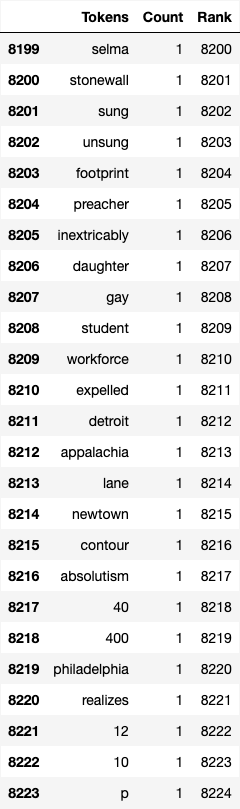
\includegraphics[width=0.35\textwidth]{figures/df_last25_stopwords.png}
    \caption{Last 25 words (inclduing stopwords) with their count.}
    \label{fig:FigLast25Stop}
\end{figure}

Using the \texttt{matplotlib.pyploy} library, a bar graph depicted in figure \ref{fig:FigBar} shows 
the top 40 words. It must be noted that the y-axis has been set to a log scale to better understand
the generated output. Although a normal bar plot without a log scale did produce a readable graph,
the difference between frequencies was not as apparent. This graph was generated using all 
options except \texttt{--stem}.

\begin{figure}[H]
    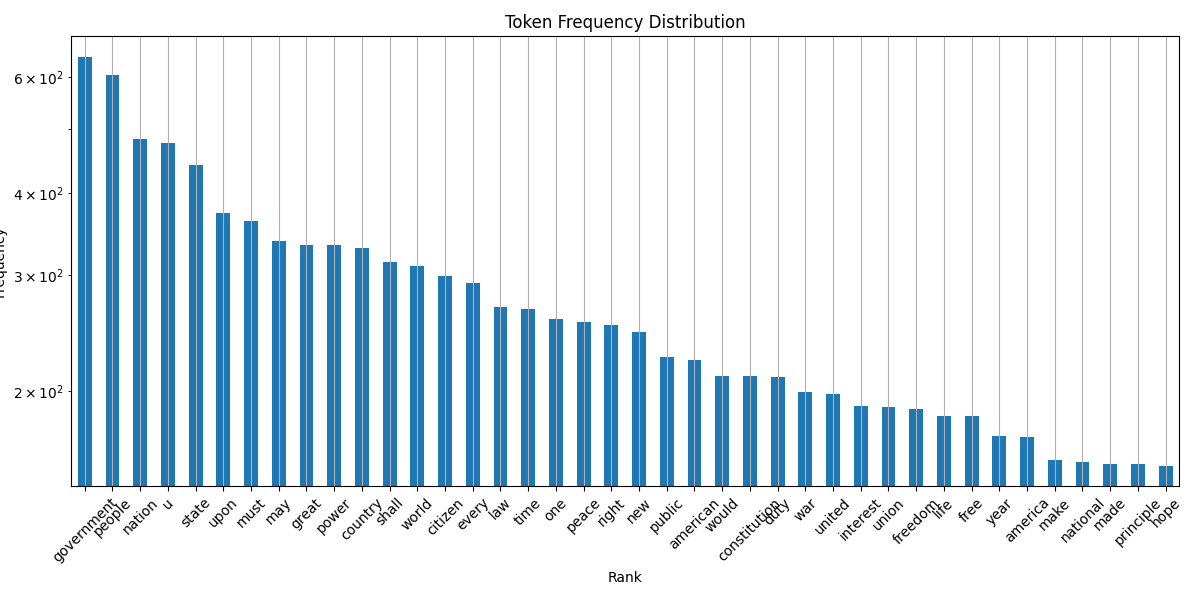
\includegraphics[width=\textwidth]{figures/bar_plot.png}
    \caption{Bar plot showing the frequencies of top 45 words.}
    \label{fig:FigBar}
\end{figure}

To better compare the output with Zipf's Law, a line graph as shown in figure \ref{fig:FigLine} has 
been generated. It must be noted that this is a log-log plot. This graph was generated using all 
options except \texttt{--stem}.

\begin{figure}[H]
    \centering
    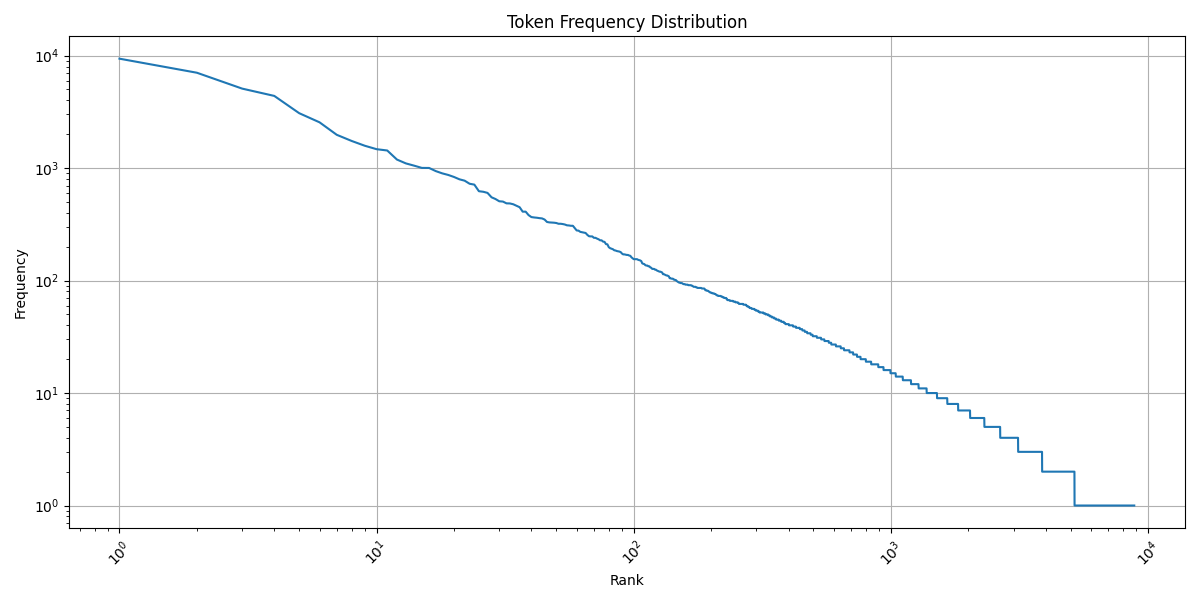
\includegraphics[width=\textwidth]{figures/line_plot.png}
    \caption{Line plot showing the words and their frequencies.}
    \label{fig:FigLine}
\end{figure}

\section{Discussion}
This section outlines common findings and insights dervided from the program.
\subsection{Findings}
On comparsion of the two bar graphs shown in figures \ref{fig:FigBar} and \ref{fig:FigBarStop}, it 
can be noticed that prior to removing stopwords, all top 40 words consist of stopwords. Once this 
normalization step has been implemented, however, words truly depicting the contents of the speech 
start populating the top 40 ranks. The other end of the list, in both the figures \ref{fig:FigLast25}
and \ref{fig:FigLast25Stop} show similar words but with different ranks as the list progresses.\\

To better compare my reuslts with those mentioned in the article, I generated line plots shown in 
figures \ref{fig:FigLine} and \ref{fig:FigLineStop}. Figure \ref{fig:FigLineStop} is very similar 
to the plots shown in the article and the similarity can be explained by the fact that this list 
inclduing stopwords complies with Zipf's Law. Figure \ref{fig:FigLine} however looks somewhat different 
as all stopwords have been reduced thereby removing the compliance with Zipf's Law.\\

As mentioned earlier, this means that removing stopwords significantly reduces the total number of 
tokens because they tend to occur frequently. In contrast, removing content words has a smaller
impact on token counts but affects the semantic richness of the text more, as content words carry meaning.

\subsection{Reflection}

\section{Appendix}
This section icnludes extra figures that might be relevant to the report but have not been referenced 
in the content.

\begin{figure}[H]
    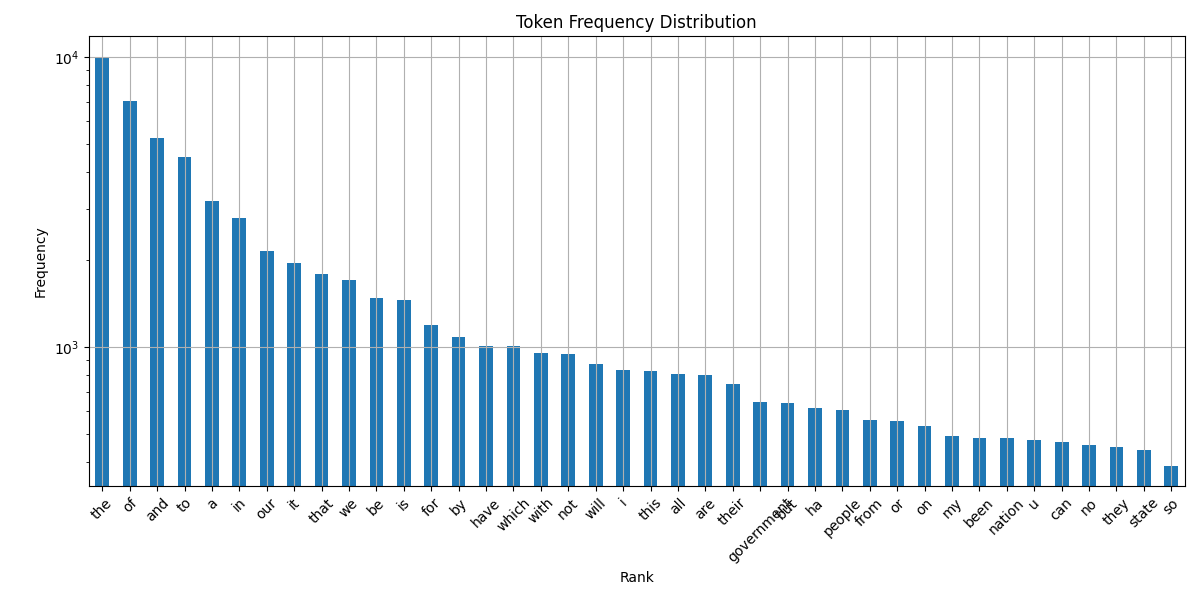
\includegraphics[width=\textwidth]{figures/bar_plot_stopwords.png}
    \caption{Bar plot showing the frequencies of top 40 words (including stopwords).}
    \label{fig:FigBarStop}
\end{figure}

\begin{figure}[H]
    \centering
    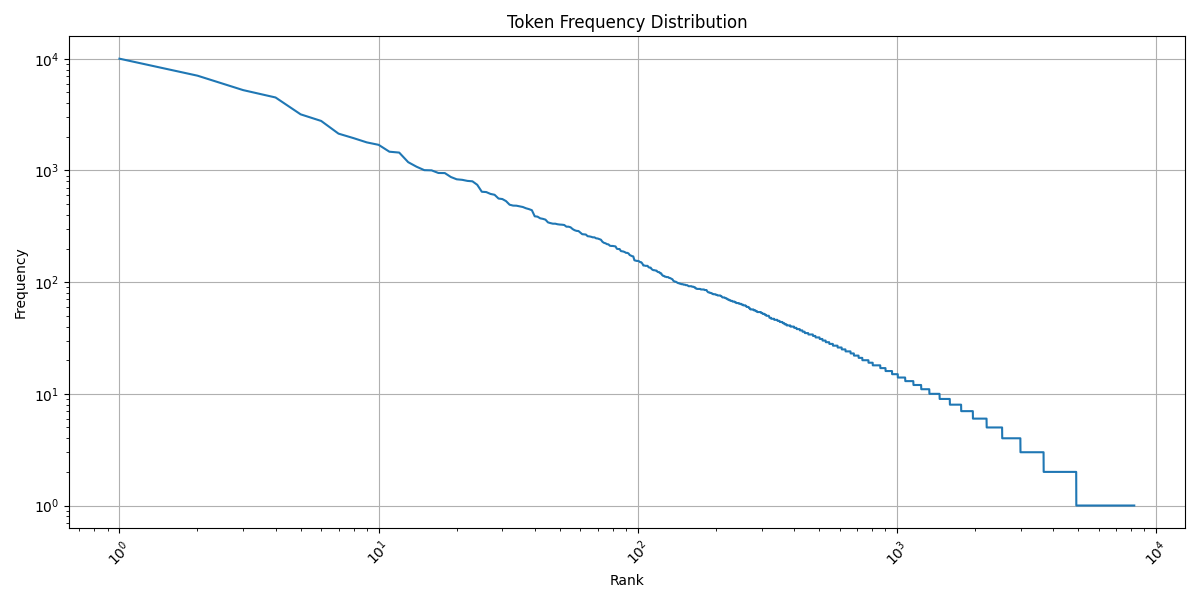
\includegraphics[width=\textwidth]{figures/line_plot_stopwords.png}
    \caption{Line plot showing the words (including stopwords) and their frequencies.}
    \label{fig:FigLineStop}
\end{figure}


\end{document}